\documentclass[aspectratio=169,10pt]{beamer}
\usepackage[utf8]{inputenc}
\usepackage[T1]{fontenc}
\usepackage[brazil]{babel}
\usepackage{amsmath,amssymb}
\usepackage{booktabs}
\usepackage{graphicx}
\graphicspath{{figs/}}

\usetheme{Madrid}
\setbeamertemplate{navigation symbols}{}

\title[Segmentação no Gray-Scott]{Segmentação 2D de padrões no Gray-Scott (The Well)}
\subtitle{Trabalho P2 de PDI --- andamento do projeto}
\author{Equipe Gray-Scott}
\institute{UFMA}
\date{Novembro de 2026}

\begin{document}

\begin{frame}
  \titlepage
\end{frame}

% ------------------------------------------------------------
\begin{frame}{Objetivo e dataset}
  \begin{columns}[T]
    \begin{column}{0.55\textwidth}
      \textbf{Pergunta:} onde estão as estruturas e como evoluem no tempo?
      \begin{itemize}
        \item Segmentação 2D dos padrões de Turing.
        \item 10 pré (P1--P10) $\times$ 3 redes (U-Net, SegFormer, Mask2Former) $\times$ 10 pós (Q1--Q10) = 300 combinações.
        \item Quatro condições: sem pré/pós, só pré, só pós, pré + pós.
        \item Dados: campos $A$ e $B$, $128 \times 128$, periódicos, 1001 instantes, 1200 trajetórias.
      \end{itemize}
      \[
      \partial_t B = \delta_B \Delta B + AB^2 - (f+k)B
      \]
    \end{column}
    \begin{column}{0.4\textwidth}
      \centering
      \begin{tabular}{lcc}
        \toprule
        Regime & $f$ & $k$ \\
        \midrule
        Gliders & 0,014 & 0,054 \\
        Bubbles & 0,098 & 0,057 \\
        Maze    & 0,029 & 0,057 \\
        Worms   & 0,058 & 0,065 \\
        Spirals & 0,018 & 0,051 \\
        Spots   & 0,030 & 0,062 \\
        \bottomrule
      \end{tabular}
    \end{column}
  \end{columns}
\end{frame}

% ------------------------------------------------------------
\begin{frame}{Situação do projeto}
  \centering
  \begin{tabular}{lc}
    \toprule
    Etapa & Situação \\
    \midrule
    1. Auditoria do dataset & \textbf{concluída} \\
    2. Ground truth & \textbf{aguarda professor} \\
    3. Software \quad 4. Piloto \quad 5. Experimentos & pendentes \\
    6. Tabelas & rascunho da tabela visual \\
    7. Artigo & pendente \\
    \bottomrule
  \end{tabular}

  \vspace{0.8em}
  \small Treinos no Colab/Kaggle (máquina local sem GPU).
\end{frame}

% ------------------------------------------------------------
\begin{frame}{Auditoria: principais achados}
  \begin{columns}[T]
    \begin{column}{0.48\textwidth}
      \small
      \begin{itemize}
        \item Divisão oficial: \textbf{160 / 20 / 20} trajetórias por regime.
        \item Leitura parcial dos HDF5: cerca de 2,5 GB em vez de 154 GB.
        \item Trajetórias estacionárias (só Gliders e Spirals) confirmadas; o padrão some ($B \approx 0$) por volta de $t \approx 500$ s.
        \item $t = 0$ é atípico (valores fora de $[0,1]$).
        \item Erro na documentação: o correto é $+AB^2$.
      \end{itemize}
    \end{column}
    \begin{column}{0.52\textwidth}
      \centering
      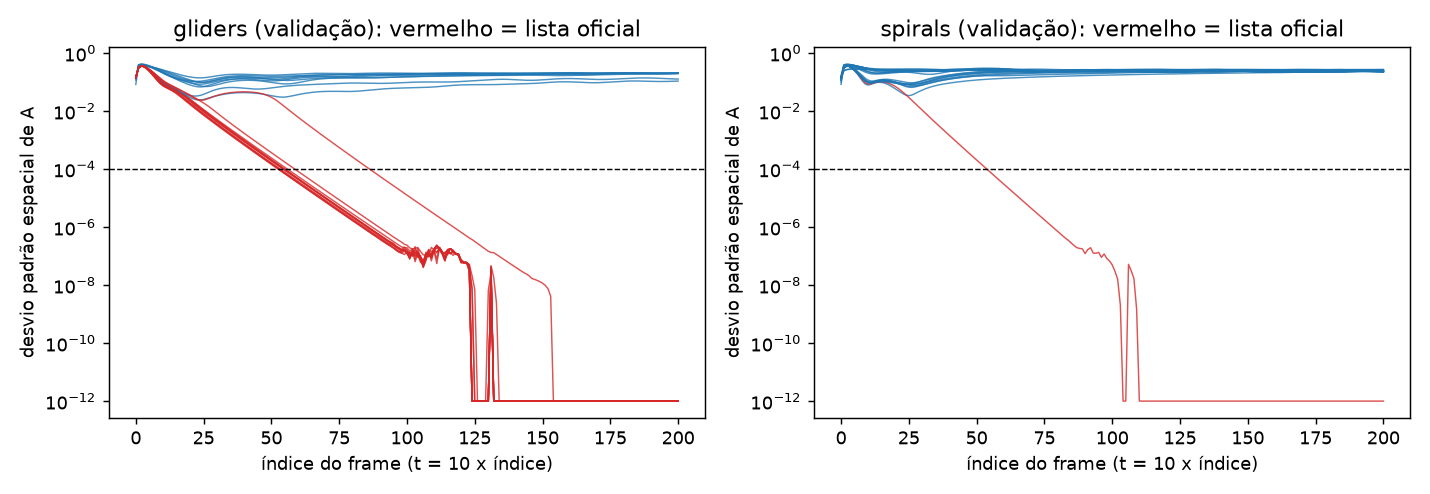
\includegraphics[width=\linewidth]{estacionarias_std_A.png}
    \end{column}
  \end{columns}
\end{frame}

% ------------------------------------------------------------
\begin{frame}{Tabela visual do fluido por instante (rascunho)}
  \begin{columns}[c]
    \begin{column}{0.38\textwidth}
      \begin{itemize}
        \item Uma trajetória por regime (linhas $A$ e $B$).
        \item $t$ = 0, 200, 400, 1000, 5000 e 10\,000 s.
        \item Maze e Spots estabilizam; Spirals e Gliders se movem até o fim.
      \end{itemize}
    \end{column}
    \begin{column}{0.62\textwidth}
      \centering
      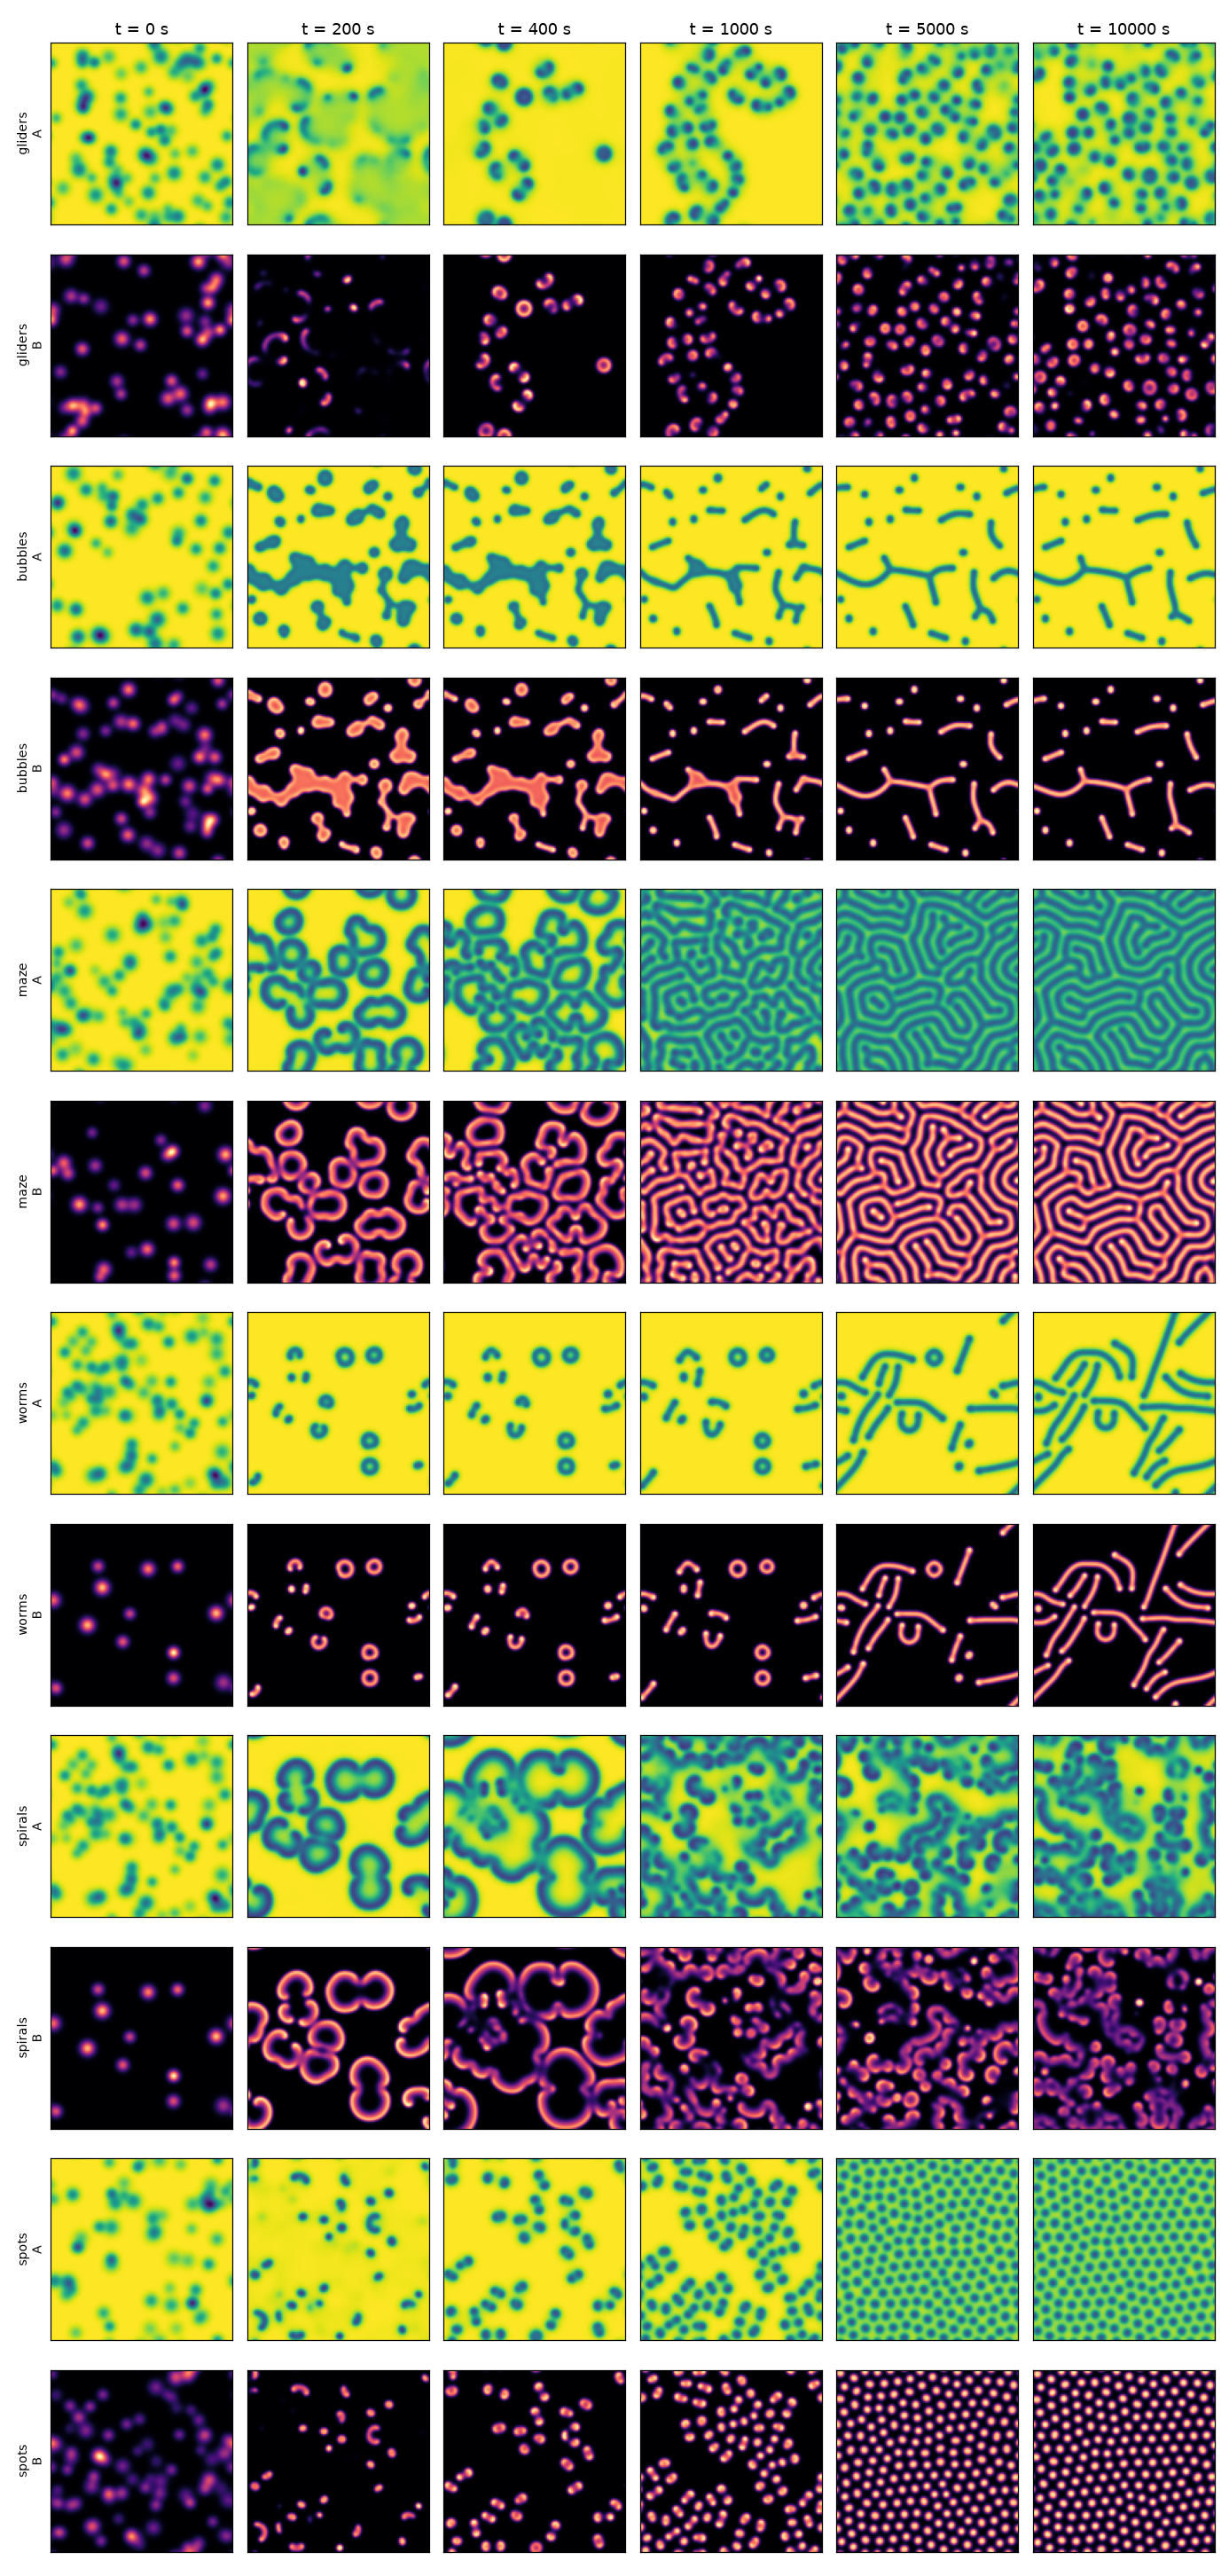
\includegraphics[height=0.88\textheight]{tabela_visual_rascunho.png}
    \end{column}
  \end{columns}
\end{frame}

% ------------------------------------------------------------
\begin{frame}{Ground truth: alternativas}
  \begin{columns}[T]
    \begin{column}{0.36\textwidth}
      \small
      \begin{enumerate}
        \item Binária: $B > \tau$ (Otsu do treino, $\tau = 0{,}151$).
        \item Três classes (com interface).
        \item Componentes conexos periódicos.
      \end{enumerate}
      Limiares ajustados só no treino.
    \end{column}
    \begin{column}{0.64\textwidth}
      \centering
      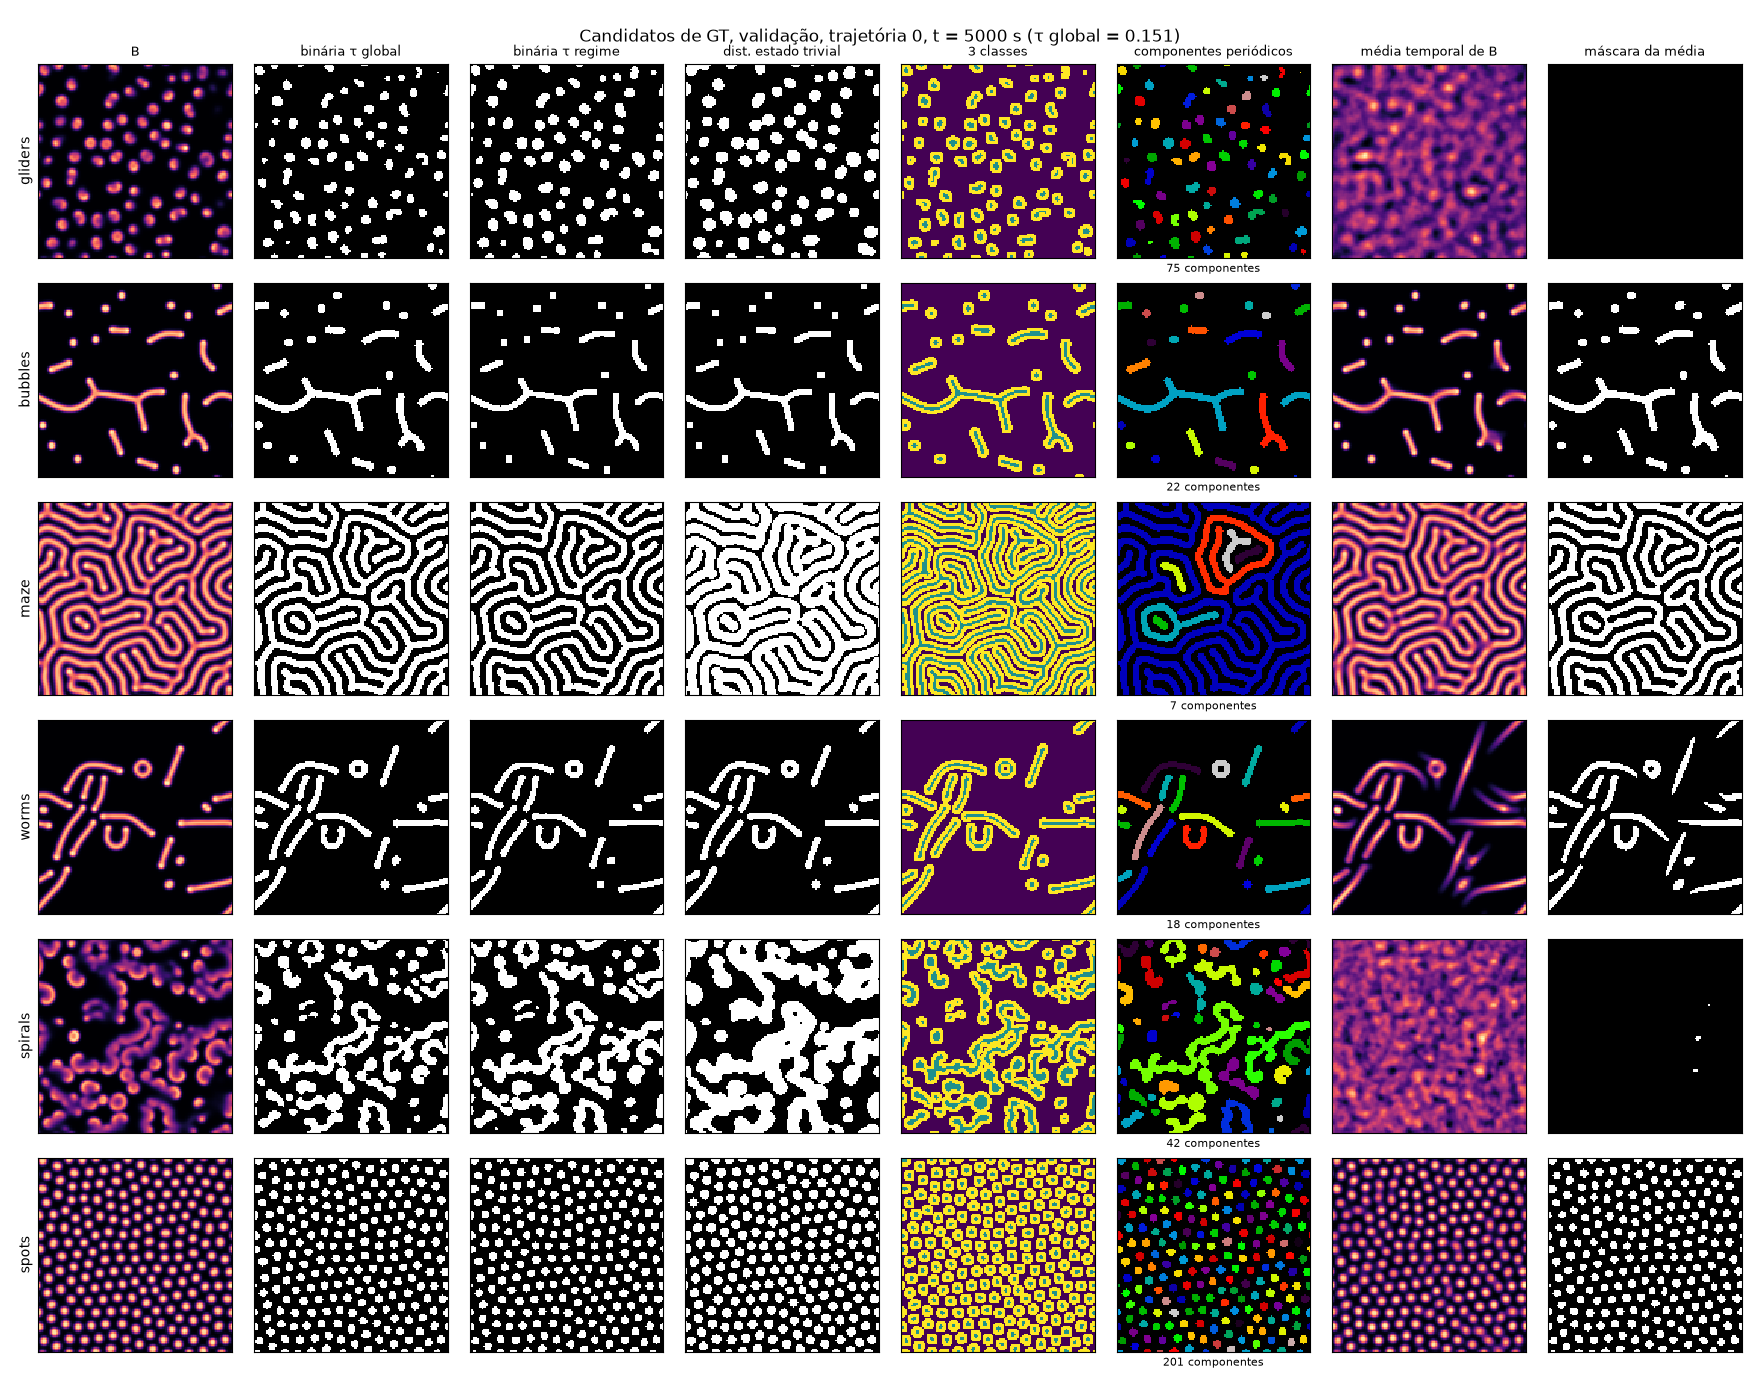
\includegraphics[width=\linewidth]{galeria_candidatos_t5000.png}
    \end{column}
  \end{columns}
\end{frame}

% ------------------------------------------------------------
\begin{frame}{O ``frame médio'' representa o fluido?}
  \centering
  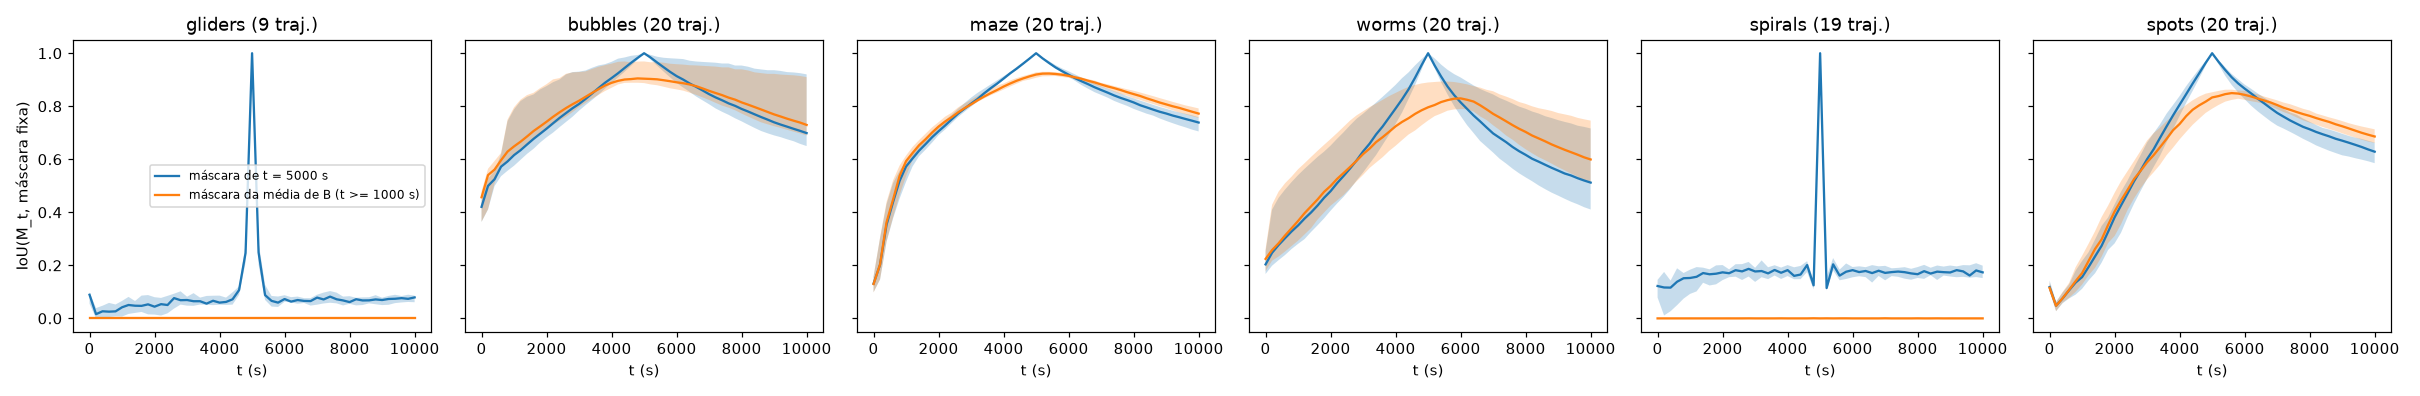
\includegraphics[width=\linewidth]{frame_medio_iou_temporal.png}

  \raggedright
  \begin{itemize}
    \item Maze, Bubbles e Spots: máscara fixa é razoável (IoU 0,6--0,9).
    \item Gliders e Spirals: padrão se move, IoU 0,08--0,17.
    \item Proposta: o frame médio define o critério; a máscara é gerada em cada frame.
  \end{itemize}
\end{frame}

% ------------------------------------------------------------
\begin{frame}{Decisões tomadas}
  \begin{itemize}
    \item \textbf{Entrada só $A$}, GT vindo de $B$, para evitar vazamento de rótulo
      (com $A$, o melhor limiar dá IoU de 0,81 a 0,98, conforme o regime).
    \item Frames sem padrão e $t = 0$ excluídos.
    \item Sem pré = dados brutos; sem pós = limiar fixo 0,5.
    \item Definição do ground truth: \textbf{aguardando o professor}.
  \end{itemize}
\end{frame}

% ------------------------------------------------------------
\begin{frame}{Perguntas ao professor e próximos passos}
  \textbf{Perguntas}
  \begin{enumerate}
    \item ``Frame médio'': instante intermediário, média de instantes ou critério aplicado a cada frame?
    \item GT por regime ou único para o fluido?
    \item Com GT estático, as métricas temporais e o Q10 continuam?
    \item O Gray-Scott (reação-difusão) é aceito como ``fluido''?
  \end{enumerate}

  \vspace{0.5em}
  \textbf{Próximos passos:} fechar o GT $\rightarrow$ código e piloto $\rightarrow$ 33 treinos $\rightarrow$ tabelas e artigo.
\end{frame}

\end{document}
